% ------- elastic plastic work -----------
\section{Elastic/plastic work} \label{work}
The elastic and plastic work can be calculated.

\begin{figure}[ht]
  \centering
  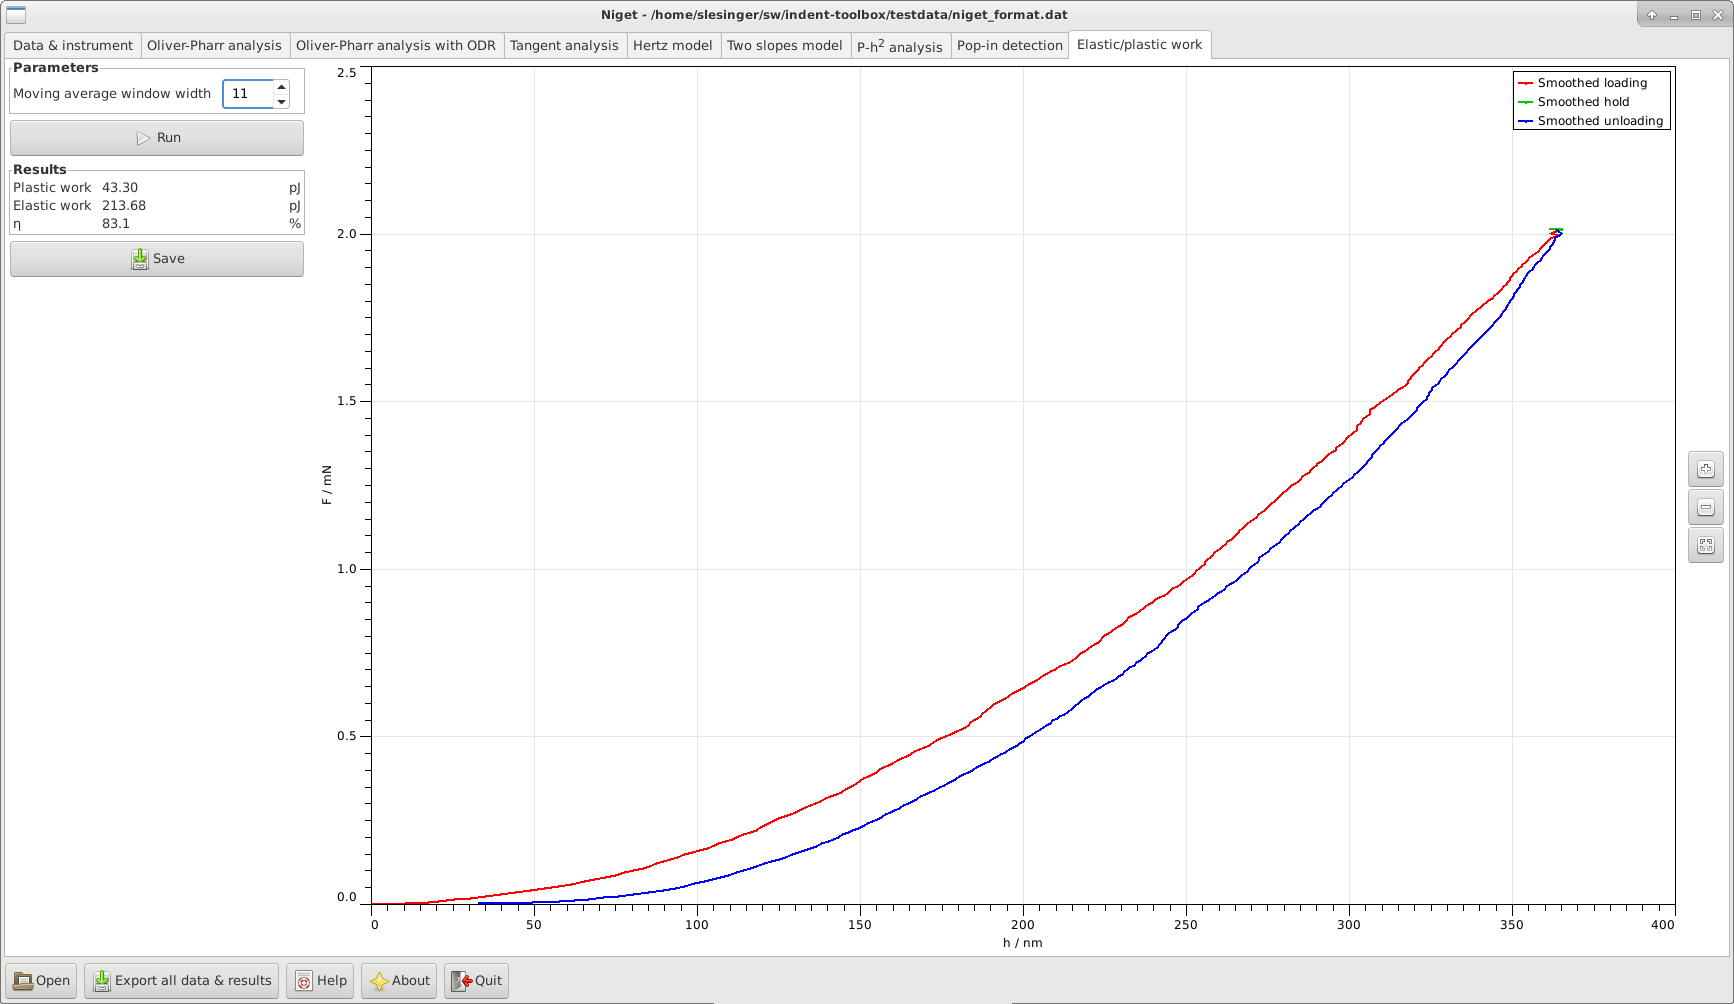
\includegraphics[width=\textwidth]{images/screen-work}
  \caption{Elastic and plastic work calculation}
\end{figure}

\subsection{Window}
The window consists of several blocks:
\begin{itemize}
 \item \emph{Parameters} allows the user to set the width of the moving average window. The value~1 corresponds to no smoothing. This value is saved in settings. 
 \item \emph{Run}  perform calculation and display curve, see section \ref{Ph2_calc}. 
 \item \emph{Save} save parameters and results to given file. 
 \item \emph{Graph}  display the (smoothed) indentation curve. 
 Stepwise zooming/unzooming can be performed by selecting a range with the mouse and pressing the \emph{Zoom}/ \emph{Unzoom} buttons. 
		     The graph is restored to its original size by the \emph{Restore} button. 
  \end{itemize}

\subsection{Procedure} \label{work_calc}
\begin{enumerate}
 \item 
We use a moving average with a fixed width and constant weight. This means we substitute a value with its average with $s$ values to the left and to the right, $w = 2s + 1$ 
$$
\hat{x} _i = \frac1w \sum_{j = -s}^{s} x_{i+j}.
$$
The value $w = 1$ corresponds to the original data. There is only one moving average type defined for both depth and load and for all three parts of the curve (load, unload, hold).
Increasing the value of $w$ noise becomes less influential but important small effects can get lost as well. 
\item
We use the simple trapezoidal rule for the integration of each curve
\begin{equation}
 I = \sum_{i=2}^n \frac12 (y_{i}-y_{i-1}) (x_{i}-x_{i-1}) 
\end{equation}
\item
The elastic work is the area under the unloading curve, the plastic work is the area enclosed by the whole indentation curve. The energy ratio is the ratio of the elastic work and the total work
\begin{eqnarray}
 W_{\mathrm{e}} &=& I_{\mathrm{unload}} \nonumber \\
 W_{\mathrm{p}} &=& I_{\mathrm{load}} + I_{\mathrm{hold}} - I_{\mathrm{unload}} \nonumber \\
 \eta_{\mathrm{IT}} &=& \frac{W_{\mathrm{e}}}{W_{\mathrm{e}}+ W_{\mathrm{p}}}\nonumber \\
\end{eqnarray}
\end{enumerate}

